\documentclass[11pt]{article}
\usepackage[utf8]{inputenc}
\usepackage[T1]{fontenc}
\usepackage{lmodern}
\usepackage[margin=1in]{geometry}
\usepackage{microtype}
\usepackage{graphicx}
\usepackage{booktabs}
\usepackage{array}
\usepackage{tabularx}
\usepackage{longtable}
\usepackage{float}
\usepackage{placeins}
\usepackage{xcolor}
\usepackage{caption}
\usepackage{natbib}
\usepackage[hidelinks]{hyperref}
\usepackage{fancyhdr}
\setlength{\parindent}{0pt}
\setlength{\parskip}{0.65em}
\setlength{\headheight}{14.5pt}
\renewcommand{\arraystretch}{1.15}
\definecolor{ink}{HTML}{19324A}
\definecolor{accent}{HTML}{A64B2A}
\hypersetup{colorlinks=true,linkcolor=ink,citecolor=accent,urlcolor=accent}
\pagestyle{fancy}
\fancyhf{}
\lhead{Chile BOP-Binding Audit}
\rhead{RER--VECM--TVECM}
\cfoot{\thepage}
\title{\textbf{When Does Chile's Balance-of-Payments Constraint Bind?}\\
\large A reproducible RER-controlled import-system audit, 1920--2024}
\author{Chapter 2 research pipeline}
\date{29 July 2026}
\begin{document}
\maketitle

\begin{abstract}
This report rebuilds the Chilean import-system analysis from source snapshots through a frozen release, exact split samples, formal integration-order gates, RER-controlled VECMs, observed-threshold conditional VECMs, and a triangulated balance-of-payments screening index. The legacy four-variable long-run coefficients reproduce to a maximum absolute difference of 1.03e-10. The reproduction succeeds, but the promoted machinery model does not: log gross machinery capital remains unresolved or at risk of I(2) in both 1920--1973 and 1974--2024. The machinery VECM and machinery-defined threshold VECM are therefore blocked. Reduced admissible systems find no RER-threshold effect (bootstrap $p=0.330$ before 1974 and $p=0.573$ after 1973). The resulting episode chronology is a screening device, not a validated latent-state estimator.

\vspace{0.5em}\noindent\textbf{Keywords:} Chile; balance of payments; imports; machinery; real exchange rate; VECM; threshold VECM; Kaldor; Thirlwall
\end{abstract}

\FloatBarrier
\section*{Resumen}
Este informe reconstruye el análisis chileno de importaciones desde las fuentes hasta una versión de datos congelada. La reproducción de los coeficientes heredados es exacta, pero el capital bruto de maquinaria no supera la compuerta de orden de integración en ninguna submuestra. Por tanto, el VECM de maquinaria y su versión umbral no se promueven. Los sistemas reducidos tampoco rechazan linealidad ($p=0.330$ y $p=0.573$). La cronología final triangula presión del ECT e indicadores observados y debe leerse como diagnóstico de episodios, no como fechamiento definitivo.

\FloatBarrier
\section{Introduction and verdict}

Chile's industrialization made foreign exchange a condition of productive transformation: machinery and intermediate imports expanded the productive apparatus, while weak export performance periodically restricted the capacity to finance those imports. The mechanism makes an import disequilibrium measure worth testing, but it does not authorize classifying crises from a residual alone \citep{bcch2025,alvarez2003}.

This paper examines whether the import requirement associated with non-reinvested surplus, gross machinery accumulation, distribution, and the real exchange rate yields an admissible long-run system and whether its adjustment identifies periods in which Chile's balance-of-payments constraint became binding. The answer is disciplined by the gate: the legacy relation is computationally reproducible, but gross machinery capital fails the required I(1) classification in both political-economic samples, so the central machinery VECM cannot carry the proposed inference.

The result separates replication from validation. Exact numerical reconciliation establishes that the archived calculation has been recovered; it cannot establish that the level variables form an admissible cointegrating system. The report consequently advances the reproducible data release and reduced-system diagnostics while holding the requested machinery coefficients and machinery ECT outside the paper-facing evidence.

\FloatBarrier
\section{Mechanism and identification}

Kaldor's mechanism runs from manufacturing expansion to increasing returns and productivity growth; cumulative causation then makes productive structure path dependent \citep{kaldor1967,kaldor1970}. Modern cross-country evidence supports the general manufacturing-growth mechanism but cannot identify a Chilean coefficient \citep{marconi2016}. Thirlwall's closure makes sustained growth conditional on export earnings and the income elasticity of imports, while later extensions admit capital flows and debt service \citep{thirlwall1979,thirlwall1982,morenobrid2003}. The combined theory predicts a foreign-exchange constraint on transformation, not a particular time-series rank or crisis classifier.

For Chile, the connecting mechanism is imported productive inputs. Official history records that CORFO-led industrialization raised capital- and intermediate-goods imports from the late 1940s, while export stagnation left insufficient foreign exchange and produced the 1961 balance-of-payments crisis \citep{bcch2025}. Plant-level analysis also emphasizes technology embodied in imported capital and intermediate goods and their limited domestic substitutability \citep{alvarez2003}. These findings make the import--machinery relation substantively grounded; they do not permit its stochastic properties to be assumed.

The post-1974 split is also substantive. Trade reform changed manufacturing composition and productivity, import penetration weakened domestic interindustry linkages, and Chile's development remained tied to copper and externally exposed structural change \citep{ffd1983a,ffd1983b,ffd2002,albala2006,palma2019,solimano2024}. A direct Chilean application of balance-of-payments-constrained growth covers 1980--2019 but cannot adjudicate the earlier system or the 1961 benchmark \citep{yunga2022}. The 1920--1973 and 1974--2024 estimates therefore represent distinct political-economic systems rather than an arbitrary mechanical partition.

\FloatBarrier
\section{Ordered data architecture}

The pipeline enforces the sequence source snapshots $\rightarrow$ canonical panel $\rightarrow$ base-year and splice audit $\rightarrow$ frozen release $\rightarrow$ integration gates $\rightarrow$ split VECM $\rightarrow$ conditional threshold test $\rightarrow$ BOP screening state $\rightarrow$ report. No downstream stage repairs an upstream object, and every estimator consumes the frozen release.

GDP, imports, investment, non-reinvested surplus, and gross machinery capital are documented in 2003 CLP. The monthly Banco Central RER series is annualized by arithmetic mean and rebased from its 1986 reference to the ClioLab 2003 scale. Table~\ref{tab:rer} shows that the splice passes every declared audit while retaining a measurable source transition.

\begin{table}[H]
\centering
\caption{RER splice and base-year audit}
\label{tab:rer}
\begin{tabular}{p{5.7cm}p{2.2cm}p{6.1cm}}
\toprule
\textbf{Audit object} & \textbf{Result} & \textbf{Verdict} \\
\midrule
Level correlation, 1986--2010 & 0.825 & Passes the declared 0.80 floor; definitions are related, not identical. \\
Growth correlation, 1987--2010 & 0.750 & Common annual movement is strong enough for a documented splice. \\
Median absolute level gap & 9.34\% & The gap is material and remains part of the sensitivity analysis. \\
2011 boundary log growth & 0.133 & The boundary passes the overlap-variance rule but is not described as seamless. \\
Coverage & 1920--2024 & One annual row per year; exact split samples are preserved. \\
\bottomrule
\end{tabular}
\end{table}

\begin{figure}[H]
\centering
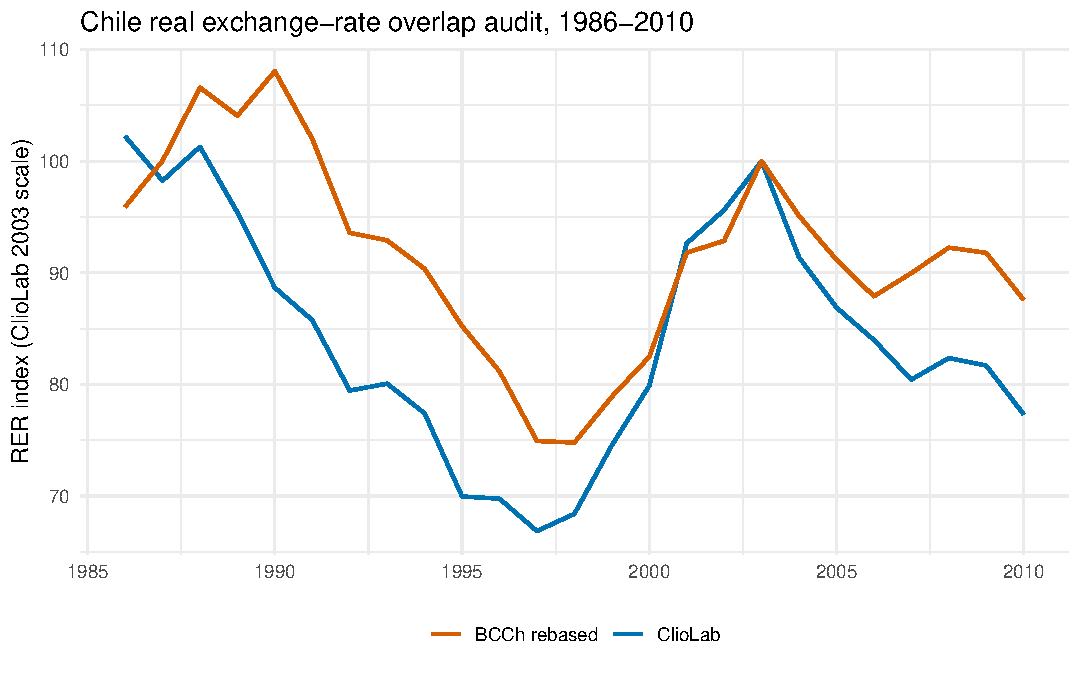
\includegraphics[width=0.92\textwidth]{figures/rer_overlap.pdf}
\caption{ClioLab and Banco Central real exchange-rate series on the 2003 scale.}
\label{fig:rer}
\end{figure}

\FloatBarrier
\section{Split-sample VECM audit}

The motivating long-run relation is
\[
\log M_t = \alpha + \beta_K k_t^{ME} +
\beta_{NRS}\log NRS_t + \beta_{\omega}\omega_t +
\beta_R\log RER_t + e_t ,
\]
where $M_t$ is real imports, $NRS_t=\Pi_t-I_t$, $k_t^{ME}$ is log gross machinery and equipment, and $\omega_t$ is the wage share. This equation is a candidate cointegrating relation only when the level variables pass the integration gate.

Table~\ref{tab:iorder} rejects promotion of the requested system. Gross machinery capital remains unresolved or at risk of I(2) in both samples. The pre-1974 wage share is I(0) and enters as a stationary control; the post-1974 RER produces mixed level evidence and is held outside the promoted long-run state. Rank selection cannot repair these failures because the variable set must be admissible before the Johansen estimator is selected.

\begin{table}[H]
\centering
\caption{Integration-order gate and estimator disposition}
\label{tab:iorder}
\footnotesize
\begin{tabular}{p{1.8cm}p{3.1cm}p{3.0cm}p{5.1cm}}
\toprule
\textbf{Sample} & \textbf{Variable} & \textbf{Classification} & \textbf{Disposition} \\
\midrule
1920--1973 & log real imports & I(1) & promoted to cointegrating state \\
1920--1973 & log gross machinery capital & unresolved or I(2) risk & held out of promoted long run system \\
1920--1973 & log non-reinvested surplus & I(1) & promoted to cointegrating state \\
1920--1973 & wage share & I(0) & stationary control \\
1920--1973 & log real exchange rate & I(1) & promoted to cointegrating state \\
1974--2024 & log real imports & I(1) & promoted to cointegrating state \\
1974--2024 & log gross machinery capital & unresolved or I(2) risk & held out of promoted long run system \\
1974--2024 & log non-reinvested surplus & I(1) & promoted to cointegrating state \\
1974--2024 & wage share & I(1) & promoted to cointegrating state \\
1974--2024 & log real exchange rate & mixed level evidence I(1) risk & held out of promoted long run system \\
\bottomrule
\end{tabular}
\end{table}

The archived four-variable coefficients reproduce exactly, with a maximum absolute difference of 1.03e-10. This result resolves the computational provenance question: the new release and code recover the legacy calculation. The same evidence rejects a stronger verdict because exact reproduction does not transform an unresolved machinery series into an I(1) state.

\begin{figure}[H]
\centering
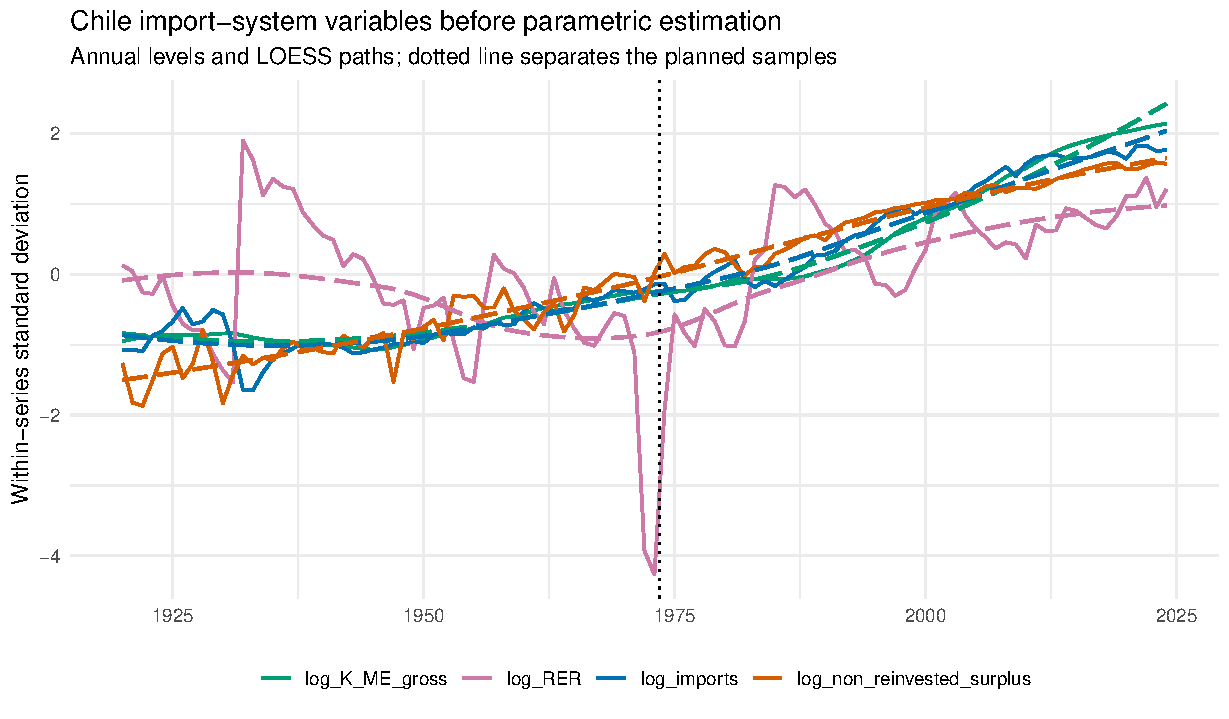
\includegraphics[width=0.96\textwidth]{figures/raw_system.pdf}
\caption{Split-sample levels and local trends for the import-system variables.}
\label{fig:raw}
\end{figure}

\FloatBarrier
\section{Conditional threshold test}

The requested import--machinery threshold VECM is blocked by the same integration gate. The reported nonlinear exercise is a reduced conditional system: imports, non-reinvested surplus, and RER form the pre-1974 state with an I(0) wage-share control; imports, non-reinvested surplus, and wage share form the post-1974 state with stationary $\Delta\log RER_t$ as a control. The observed threshold variable is annual $\Delta\log RER_t$, and the import ECT does not define its own regime.

The 15\% trimmed search evaluates 160 candidates, imposes minimum regime sizes, and uses 999 conditional residual bootstrap replications in each sample. Table~\ref{tab:threshold} shows that neither sample rejects a linear adjustment process. The threshold estimates therefore locate descriptive profile minima; they do not identify statistically distinct crisis regimes.

\begin{table}[H]
\centering
\caption{Observed-RER threshold tests}
\label{tab:threshold}
\footnotesize
\begin{tabular}{p{2.2cm}p{1.8cm}p{3.2cm}p{1.4cm}p{1.7cm}p{2.2cm}}
\toprule
\textbf{Sample} & \textbf{Threshold} & \textbf{Profile interval} & \textbf{LR} & \textbf{Bootstrap p} & \textbf{Verdict} \\
\midrule
1920--1973 & -0.092 & [-0.097, 0.046] & 3.270 & 0.330 & No threshold effect \\
1974--2024 & -0.042 & [-0.050, 0.078] & 2.246 & 0.573 & No threshold effect \\
\bottomrule
\end{tabular}
\end{table}

\begin{figure}[H]
\centering
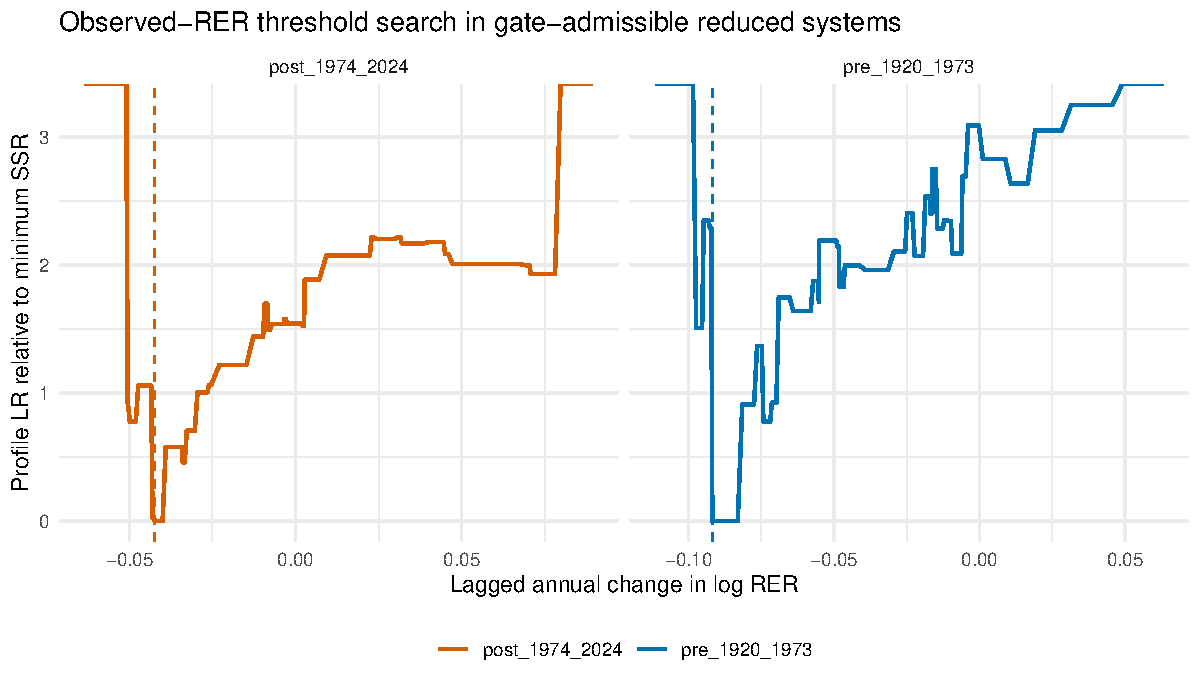
\includegraphics[width=0.92\textwidth]{figures/threshold_profile.pdf}
\caption{Trimmed threshold-search objective profiles.}
\label{fig:threshold}
\end{figure}

\FloatBarrier
\section{Balance-of-payments screening state}

The reduced-system ECT is normalized on imports:
\[
ECT_{M,t}=\log M_t-\widehat{\log M_t},
\qquad B^{ECT}_t=-ECT_{M,t}.
\]
A positive $B^{ECT}_t$ records imports below the reduced-system requirement. The screening index combines standardized ECT pressure with current-account pressure, the goods balance, and manufactured-import compression. Confirmed binding requires ECT pressure of at least one robust standard deviation and at least one observed BOP signal; disagreement remains visible as ECT-only or observed-only pressure.

Table~\ref{tab:episodes} lists the confirmed runs. The concentration in the 1950s and the immediate post-1973 years is historically plausible, but plausibility is not validation. The classifier does not confirm the officially documented 1961 crisis, and that false negative is decisive: the index organizes evidence but cannot supply a definitive chronology.

\begin{table}[H]
\centering
\caption{Confirmed binding runs in the triangulation screen}
\label{tab:episodes}
\begin{tabular}{p{2.5cm}p{2.5cm}p{2.2cm}p{2.2cm}p{3.0cm}}
\toprule
\textbf{Sample} & \textbf{Run} & \textbf{Duration} & \textbf{Peak year} & \textbf{Peak index} \\
\midrule
1920--1973 & 1953--1955 & 3 & 1954 & 1.430 \\
1920--1973 & 1958--1958 & 1 & 1958 & 1.292 \\
1920--1973 & 1973--1973 & 1 & 1973 & 0.974 \\
1974--2024 & 1975--1976 & 2 & 1976 & 0.659 \\
1974--2024 & 1978--1979 & 2 & 1979 & 1.179 \\
\bottomrule
\end{tabular}
\end{table}

\begin{figure}[H]
\centering
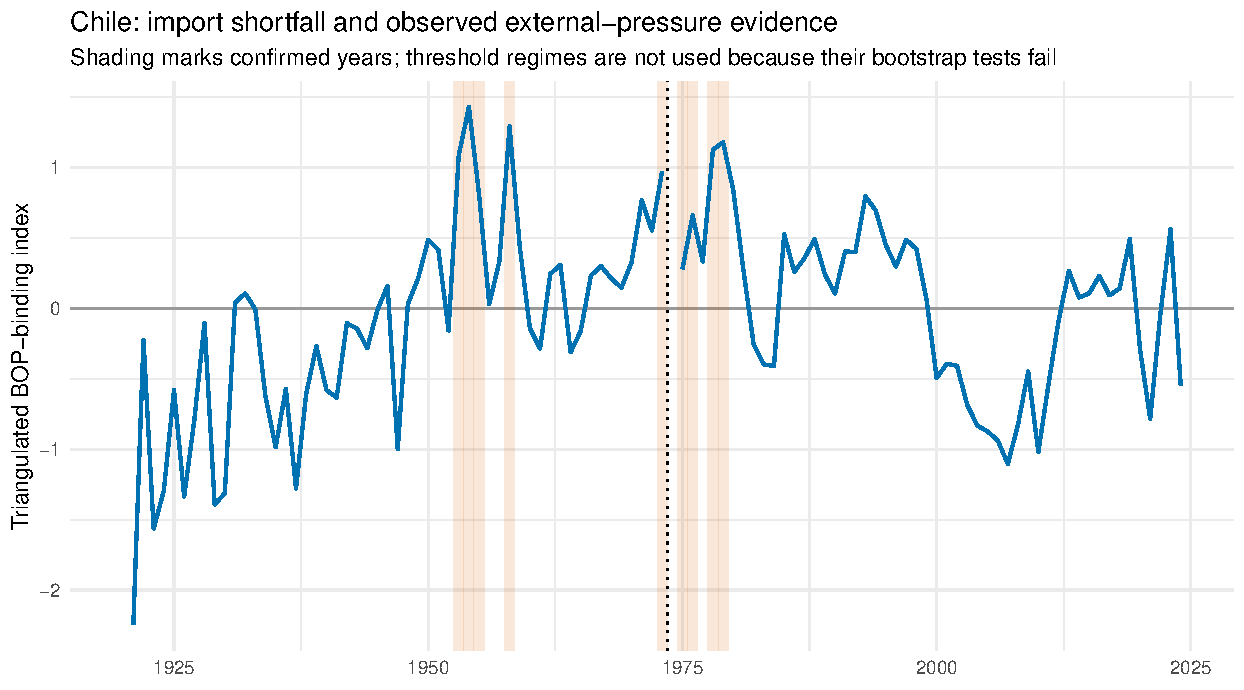
\includegraphics[width=0.82\textwidth]{figures/binding_index.pdf}
\caption{Triangulated balance-of-payments screening index and classification.}
\label{fig:binding}
\end{figure}

\begin{figure}[H]
\centering
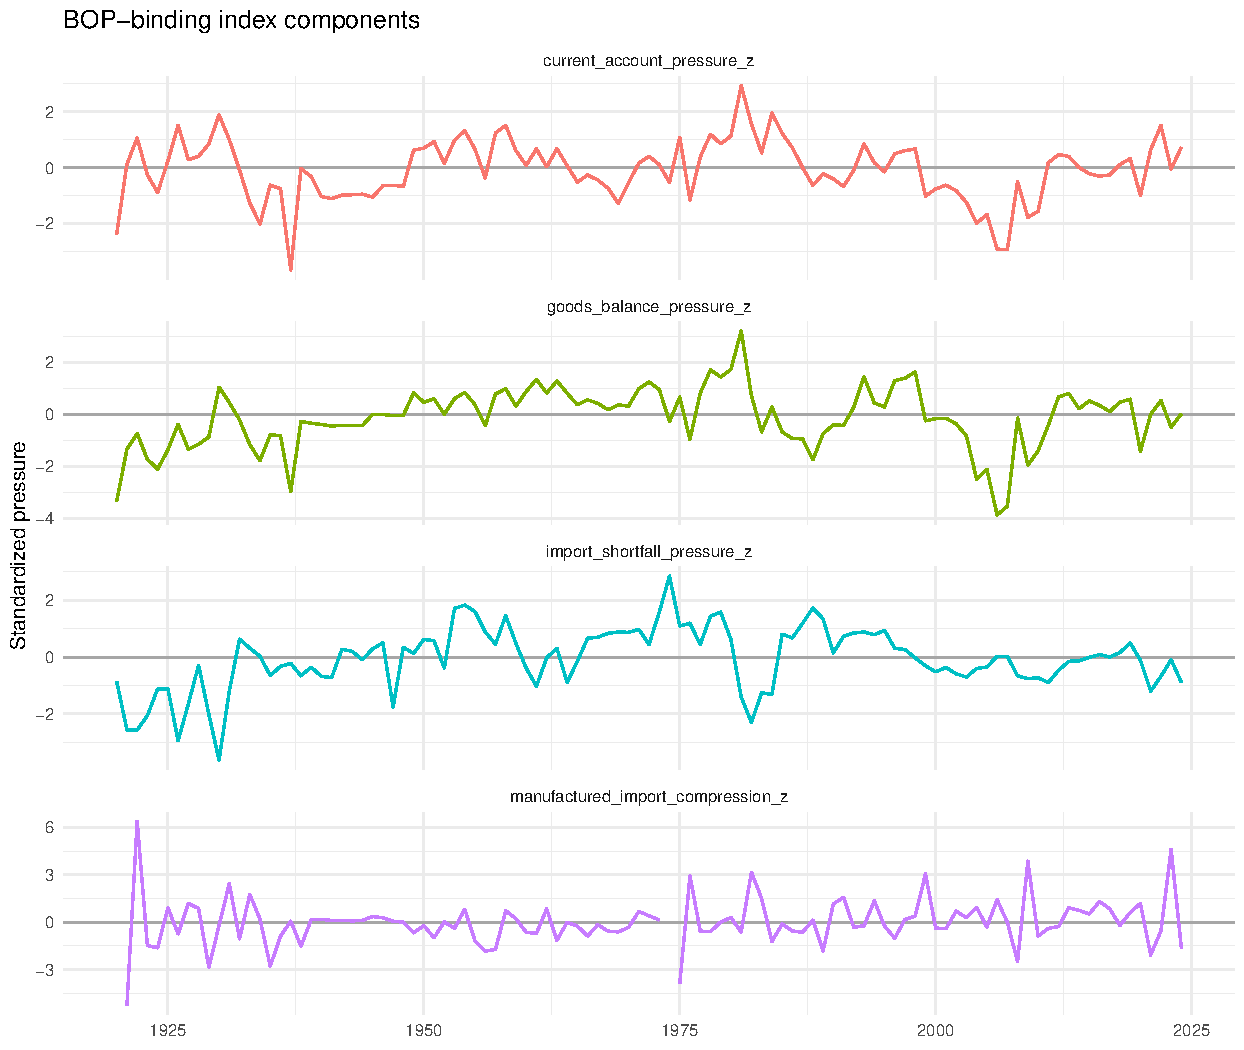
\includegraphics[width=0.82\textwidth]{figures/binding_components.pdf}
\caption{Model-based and observed components of the screening index.}
\label{fig:components}
\end{figure}

\FloatBarrier
\section{Robustness and specification space}

The robustness stage covers alternative RER splice dates, ClioLab-only and spliced RER inputs, deterministic terms, lag orders, adjacent sample boundaries, the 999-replication threshold bootstrap, leave-one-episode-out checks, condition-number reporting, and confidence-band overlap. These exercises expose sensitivity without using decimal equality as a gate. The machinery model remains blocked throughout; stability of a held coefficient cannot substitute for integration admissibility.

The reduced Johansen ranks retain asymptotic trace evidence as a descriptive input because each split exceeds 30 annual observations. A machinery-rank bootstrap is not reported because the machinery estimator is blocked before rank promotion. This omission is a governed result rather than missing computation: bootstrap refinement cannot rescue a state vector rejected by the upstream gate.

Alternative observed threshold variables reveal reduced-system nonlinearity that the RER-change threshold does not. Current-account pressure rejects linearity in both samples, and annual financing-pressure change rejects only before 1974. Table~\ref{tab:altthreshold} reports the 999-replication results. Because current-account pressure is itself an observed BOP outcome, the test conditions ECT adjustment but cannot independently validate a chronology that also uses external-account evidence.

\begin{table}[H]
\centering
\caption{Alternative observed threshold variables in reduced systems}
\label{tab:altthreshold}
\footnotesize
\begin{tabular}{p{2.2cm}p{4.2cm}p{2.3cm}p{2.1cm}p{2.8cm}}
\toprule
\textbf{Sample} & \textbf{Threshold variable} & \textbf{Estimate} & \textbf{Bootstrap p} & \textbf{Verdict} \\
\midrule
1920--1973 & Current-account pressure & 0.053 & 0.035 & Reject linearity \\
1974--2024 & Current-account pressure & -0.001 & 0.039 & Reject linearity \\
1920--1973 & Annual financing-pressure change & 0.008 & 0.048 & Reject linearity \\
1974--2024 & Annual financing-pressure change & 0.019 & 0.519 & Do not reject \\
\bottomrule
\end{tabular}
\end{table}

The discrete financing-compression indicator contains only 1 pre-1974 episode observation and 3 post-1973 observations after lag alignment. Both regimes fail the minimum size of ten, so no binary-regime estimator or bootstrap is promoted.

\begin{figure}[H]
\centering
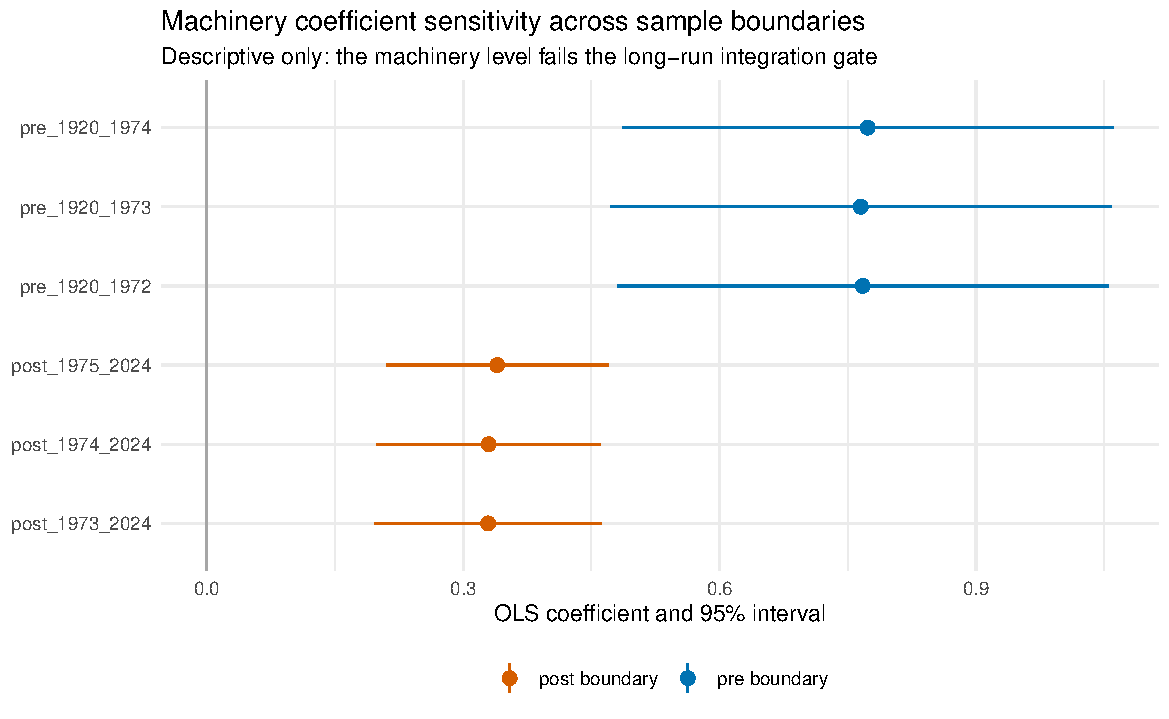
\includegraphics[width=0.95\textwidth]{figures/boundary_sensitivity.pdf}
\caption{Adjacent-boundary sensitivity for the held machinery relation.}
\label{fig:boundary}
\end{figure}

\FloatBarrier
\section{Conclusion}

The rebuild succeeds as an audit and rejects the central econometric shortcut. Chile's imported-machinery and foreign-exchange mechanism is historically coherent, but the current gross machinery series does not support the proposed split-sample machinery VECM. The reduced systems provide no formal evidence of RER-defined threshold adjustment, while current-account pressure and pre-1974 financing-pressure change condition adjustment nonlinearly. Those external-pressure thresholds are evidence about the adjustment mechanism, not independent confirmation of binding dates. The report therefore retains the BOP index as a transparent screening panel and directs the next research step toward resolving the machinery stock's stochastic properties and validating crisis dates against independent historical records.

The empirical verdict changes the report's contribution. It no longer claims to have estimated when the external constraint became binding from a machinery ECT; it demonstrates which parts of that claim reproduce, which parts pass stochastic gates, and where the evidence fails. That distinction preserves the Kaldorian question while preventing a generated latent state from validating itself.

\FloatBarrier
\section*{Data availability and reproducibility}

The frozen modelling release is stored at \texttt{data/releases/chile\_bop\_binding\_v1/}. Every report table and figure is copied from completed stage ledgers. The report builder performs no estimation and records the SHA-256 hash of each consumed input.

\FloatBarrier
\section*{Limitations}

The annual sample is small, the RER splice joins related but non-identical source definitions, the gross machinery series fails the I(1) gate, the reduced Johansen ranks are descriptive rather than bootstrapped rank claims, and the observed BOP indicators are incomplete proxies for reserve scarcity, rationing, and access to finance. These limits bind the interpretation rather than appearing as generic qualifications.

\FloatBarrier
\section*{Declarations}

\textbf{Ethics.} The study uses historical aggregate data and involves no human subjects.

\textbf{Author contributions (CRediT).} Conceptualization, methodology, software, validation, formal analysis, data curation, visualization, and writing are documented in the repository workflow; final scholarly responsibility remains with the dissertation author.

\textbf{Funding.} No project-specific funding information was supplied.

\textbf{Conflicts of interest.} None declared.

\textbf{AI-use disclosure.} Codex assisted with reproducible code, evidence organization, diagnostics, and report assembly under human direction. All claims remain auditable against the frozen release, stage ledgers, and verified sources.

\FloatBarrier
\begin{thebibliography}{99}
\pagestyle{fancy}
\raggedright

\bibitem[Albala-Bertrand(2006)]{albala2006}
Albala-Bertrand, J. M. (2006). Changes in Chile's production structure, 1986--1996: Output and industrial interdependence. \textit{CEPAL Review, 88}, 159--172.
\url{https://repositorio.cepal.org/server/api/core/bitstreams/8b0c80bc-2006-4abb-b9ac-cc45e7fb6ba0/content}

\bibitem[Álvarez and Fuentes(2003)]{alvarez2003}
Álvarez, R., \& Fuentes, J. R. (2003). \textit{Trade reforms and manufacturing industry in Chile} (Working Paper No. 210). Banco Central de Chile.
\url{https://www.bcentral.cl/contenido/-/details/documento-de-trabajo-n-210}

\bibitem[Banco Central de Chile(2025)]{bcch2025}
Banco Central de Chile. (2025). \textit{100 años de política económica y comercio exterior de Chile}.
\url{https://www.bcentral.cl/en/w/blog/100-anios-de-politica-economica-y-comercio-exterior-de-chile}

\bibitem[Ffrench-Davis(1983a)]{ffd1983a}
Ffrench-Davis, R. (1983a). El experimento monetarista en Chile: Una síntesis crítica. \textit{Desarrollo Económico, 23}(90), 163--196.
\url{https://doi.org/10.2307/3466468}

\bibitem[Ffrench-Davis(1983b)]{ffd1983b}
Ffrench-Davis, R. (1983b). Deuda externa y balanza de pagos de América Latina: Tendencias recientes y perspectivas. \textit{Estudios Internacionales, 16}(62), 281--304.
\url{https://doi.org/10.5354/0719-3769.1983.16673}

\bibitem[Ffrench-Davis(2002)]{ffd2002}
Ffrench-Davis, R. (2002). \textit{Economic reforms in Chile: From dictatorship to democracy}. University of Michigan Press.
\url{https://doi.org/10.3998/mpub.17208}

\bibitem[Kaldor(1967)]{kaldor1967}
Kaldor, N. (1967). \textit{Strategic factors in economic development}. Cornell University.
\url{https://books.google.com/books?id=\_IgeAAAAMAAJ}

\bibitem[Kaldor(1970)]{kaldor1970}
Kaldor, N. (1970). The case for regional policies. \textit{Scottish Journal of Political Economy, 17}(3), 337--348.
\url{https://doi.org/10.1111/j.1467-9485.1970.tb00712.x}

\bibitem[Marconi et al.(2016)]{marconi2016}
Marconi, N., Reis, C. F. de B., \& Araújo, E. C. de. (2016). Manufacturing and economic development: The actuality of Kaldor's first and second laws. \textit{Structural Change and Economic Dynamics, 37}, 75--89.
\url{https://doi.org/10.1016/j.strueco.2015.12.002}

\bibitem[Moreno-Brid(2003)]{morenobrid2003}
Moreno-Brid, J. C. (2003). Capital flows, interest payments and the balance-of-payments constrained growth model. \textit{Metroeconomica, 54}(2--3), 346--365.
\url{https://doi.org/10.1111/1467-999X.00170}

\bibitem[Palma(2019)]{palma2019}
Palma, J. G. (2019). Desindustrialización, desindustrialización ``prematura'' y ``síndrome holandés''. \textit{El Trimestre Económico, 86}(344), 901--966.
\url{https://doi.org/10.20430/ete.v86i344.970}

\bibitem[Solimano and Zapata-Román(2024)]{solimano2024}
Solimano, A., \& Zapata-Román, G. (2024). \textit{Chilean economic development under neoliberalism}. Cambridge University Press.
\url{https://doi.org/10.1017/9781009477352}

\bibitem[Thirlwall(1979)]{thirlwall1979}
Thirlwall, A. P. (1979). The balance of payments constraint as an explanation of international growth rate differences. \textit{PSL Quarterly Review, 32}(128), 45--53.
\url{https://doi.org/10.13133/2037-3643/12804}

\bibitem[Thirlwall and Hussain(1982)]{thirlwall1982}
Thirlwall, A. P., \& Hussain, M. N. (1982). The balance of payments constraint, capital flows and growth rate differences between developing countries. \textit{Oxford Economic Papers, 34}(3), 498--510.
\url{https://doi.org/10.1093/oxfordjournals.oep.a041565}

\bibitem[Yunga Medina et al.(2022)]{yunga2022}
Yunga Medina, F., Tapia Morquecho, C., Camacho Manzanillas, S., \& Cueva Jiménez, A. (2022). Does the balance of payments constrain economic growth? New evidence for Chile 1980--2019. \textit{Boletín de Coyuntura, 35}, 25--35.
\url{https://doi.org/10.31243/bcoyu.35.2022.1851}

\end{thebibliography}
\end{document}

